\chapter{Determination of Rare Earth Elements in Hypersaline Solutions Using Low-Volume, Liquid-Liquid Extraction}
\chaptermark{LLE method for brines}

This chapter is adapted from a publication by the same name, co-authored by David A. Dzombak and Athanasios K. Karamalidis.
This paper is citable as: 

Noack, C. W.; Dzombak, D. A.; Karamalidis, A. K., Determination of Rare Earth Elements in Hypersaline Solutions Using Low-Volume, Liquid-Liquid Extraction. \textit{Environ. Sci. Technol.} \textbf{2015}, \textit{Article ASAP}, DOI: 10.1021/acs.est.5b00151

My contributions to this work were the experimental design; execution of experiments including ICP-MS analysis; data analysis and visualization; interpretation of results; and drafting of the manuscript.

\clearpage

\section*{Abstract}
Complex, hypersaline brines --- including those co-produced with oil and gas, rejected from desalination technologies, or used as working fluids for geothermal electricity generation --- could contain critical materials such as the rare earth elements (REE) in valuable concentrations.
Accurate quantitation of these analytes in complex, aqueous matrices is necessary for evaluation and implementation of systems aimed at recovering those critical materials.
However, most analytical methods for measuring trace metals have not been validated for highly saline and/or chemically complex brines.
Here we modified and optimized previously published liquid-liquid extraction (LLE) techniques [Shabani et al., \textit{Anal. Chem.} 1990, 62 (24) 2709-2714; Lawrence and Kamber, \textit{Geostand. Geoanal. Res.} 2007, 31 (2) 95-103], using bis(2-ethylhexyl) phosphate as the extractant in a heptane diluent, and studied its efficacy for REE recovery as a function of three primary variables: background salinity (as NaCl), concentration of a competing species (here Fe), and concentration of dissolved organic carbon (DOC).
Results showed that the modified LLE was robust to a range of salinity, Fe, and DOC concentrations studied as well as constant, elevated Ba concentrations.
With proper characterization of the natural samples of interest, this method could be deployed for accurate analysis of REE in small volumes of hyper-saline and chemically complex brines.

\section{Introduction}

The rare earth elements (REE) are among the most frequently cited critical materials for clean energy and high-tech manufacturing \citep{APS_CritMat,USDOE_CritMat}.
The unique and varied properties of REE have led to their application in more consumer products than nearly any other element group \citep{Castor_Hedrick}.
REE are mostly obtained from mining and processing of REE-enriched ores \citep{USDOE_CritMat}.
While economically preferred, mining is laborious with a significant environmental burden, and inexpensive alternative sources of critical materials are sought after resources.

Aqueous byproduct or waste streams, both natural and industrial, are potential sources of the REE and other critical materials.
With increasing global interest in geothermal energy \citep{Lund_Geothermics_2011},
development of unconventional oil and gas resources (e.g. hydraulic fracturing of organic rich shales) \citep{EIA_2013},
and desalination technologies \citep{Shannon_Nat_2008, Elimelech_Sci_2011},
large volumes of waste brines are being managed and processed at great expense.
Development of technologies for recovery of valuable byproducts, such as the REE, from these waste streams could improve the economics of these technologies while diversifying available critical material resources.
Development of such technologies requires accurate determination of the source REE concentration in order to develop and implement recovery systems.
However, precise quantitation of REE in complex matrices like brines is a significant challenge for conventional instrumentation such as inductively coupled plasma mass spectrometry (ICP-MS) \citep{Agatemor_ACA_2011}.

There exists a dearth of methodologies in the analytical literature for quantitation of REE in brines by ICP-MS.
Many approaches have been applied for separation and concentration of REE from aqueous media including solid-phase extraction (SPE)
\citep{Benkhedda_JAAS_2001, Fu_Tal_2007, Haley_MC_2003, Halicz_JAAS_1996, Hirata_Tal_2002, Kajiya_SAB_2004, Katarina_Tal_2009, Kim_AG_2010, Kuhn_FJAC_2000, Kumar_Desal_2011, Moller_SAB_1992, Stetzenbach_GW_1994, Vicente_SAB_1998, Wen_Analyst_1999, Willie_SAB_2001, Zhang_AC_1998, Zhu_Tal_2009},
co-precipitation (co-ppt) \citep{Shaw_AC_2003, Shannon_REEinGWFS, Raso_Tal_2013},
and liquid-liquid extraction (LLE) \citep{Shabani_AC_1990, Lawrence_GGR_2007, Kimura_BCSJ_1960, Kimura_BCSJ_1961}.
However, nearly all studies in the analytical chemistry literature have focused on fresh water or seawater matrices, neglecting hypersaline waters (i.e. more concentrated than $\sim0.7$ M NaCl or seawater).
Despite this deficiency, approximately 14\% of published measurements of REE in groundwater constitute brine samples (greater than 1 eq/kg ionic strength) \citep{Noack_EST_2014}, with these analyses utilizing methodologies not explicitly validated for extreme salinity.

Commonly applied separation techniques such as SPE and co-ppt may lack the robustness necessary to analyze REE in hypersaline brines.
For example, high dissolved organic carbon may lead to fouling of column-based SPE while high dissolved metal loads may lead to saturation of the surface sites responsible for REE binding.
Oliveira et al. \citep{Oliveira_JAAS_2011} ascribed diminished Zn recovery in 166\textperthousand\ salinity produced water to competitive sorption of matrix cations on their iminodiacetate resin.
Similarly, excessive cations in hypersaline solutions may screen the REE from sorption sites during co-ppt, a phenomenon noted by Nelson et al. \citep{Nelson_ESTL_2014} for Ra determination in produced waters from the Marcellus Shale by both \ce{BaSO4} and \ce{MnO2} co-ppt.
Moreover, at the elevated pH necessary for SPE and co-ppt techniques, the formation of energetically favorable, neutral- or negatively-charged aqueous complexes of the REE (with both organic and inorganic ligands) can further limit REE-particle partitioning \citep{Erel_GCA_1993}. 

Liquid-liquid extractions are potentially robust to all of these conditions and represent an attractive alternative for REE separation from hypersaline solutions \citep{Nash_SXIX_1993}.
Since LLE of REE from highly acidic solutions has been thoroughly studied for separation of lanthanides and actinides during nuclear fuel reprocessing \citep[e.g. refs.][]{Weaver_ORNL_1964, Nilsson_SXIX_2007} elevated pH is not required of LLE techniques.
Moreover, electrolyte theory dictates that increased sample salinity should enhance chemical partitioning (through salting out of neutral/micellar REE-organic ligand complexes from the aqueous feed to the organic solvent) and physical phase separation (by collapsing the electric double layer of the organic droplets, hastening coalescence).
A primary obstacle in extraction of hydrophilic metals to a hydrophobic, organic phase is the dehydration of the metal cations in the aqueous phase.
However, increasing salt concentrations decrease the effective concentration of water in the solution available for hydration of the target metal cations (REE), improving the energetics of the extraction \citep{Nash_SXIX_1993}.

In this work, efficiency of REE separation and concentration from synthetic brines using a LLE method for quantitative analysis was studied.
The LLE method was adapted, modified, and optimized from previously published studies \citep{Shabani_AC_1990, Lawrence_GGR_2007}.
For the LLE, a common ligand used for REE complexation and extraction, bis(2-ethylhexyl) phosphate (HDEHP), was studied in a heptane diluent.
The objectives of this work were to: (1) evaluate the feasibility of REE recovery from small volumes of hypersaline solutions by LLE, (2) optimize the LLE methodology for high salinity brines, and (3) study the influence of brine composition on REE recovery.

\section{Modified liquid-liquid extraction procedure}

The modified LLE method adheres to many of the physical steps of the methods originally developed by Shabani et al. 
\citep{Shabani_AC_1990} and Lawrence and Kamber \citep{Lawrence_GGR_2007}, but following optimization, differs in the operating conditions.
A schematic flowsheet of the process is shown in Figure~\ref{fig:flowsheet}.
The process involved sample preparation, followed by three cycles of extraction, whereby the REE were complexed by the HDEHP ligand and brought into the organic phase, leaving an REE-free, waste brine.
Matrix elements were rinsed from the organic phase with dilute acid, and, finally, the REE were recovered by four cycles of elution with strong acid.
This REE-loaded aqueous phase was then analyzed by ICP-MS.
The details of the process are described in following. Details of sample preparation, instrumentation, analytical protocols, and data analysis methods are presented in Section~\ref{sec:MnM}.

\begin{sidewaysfigure}[htbp]
\begin{center}
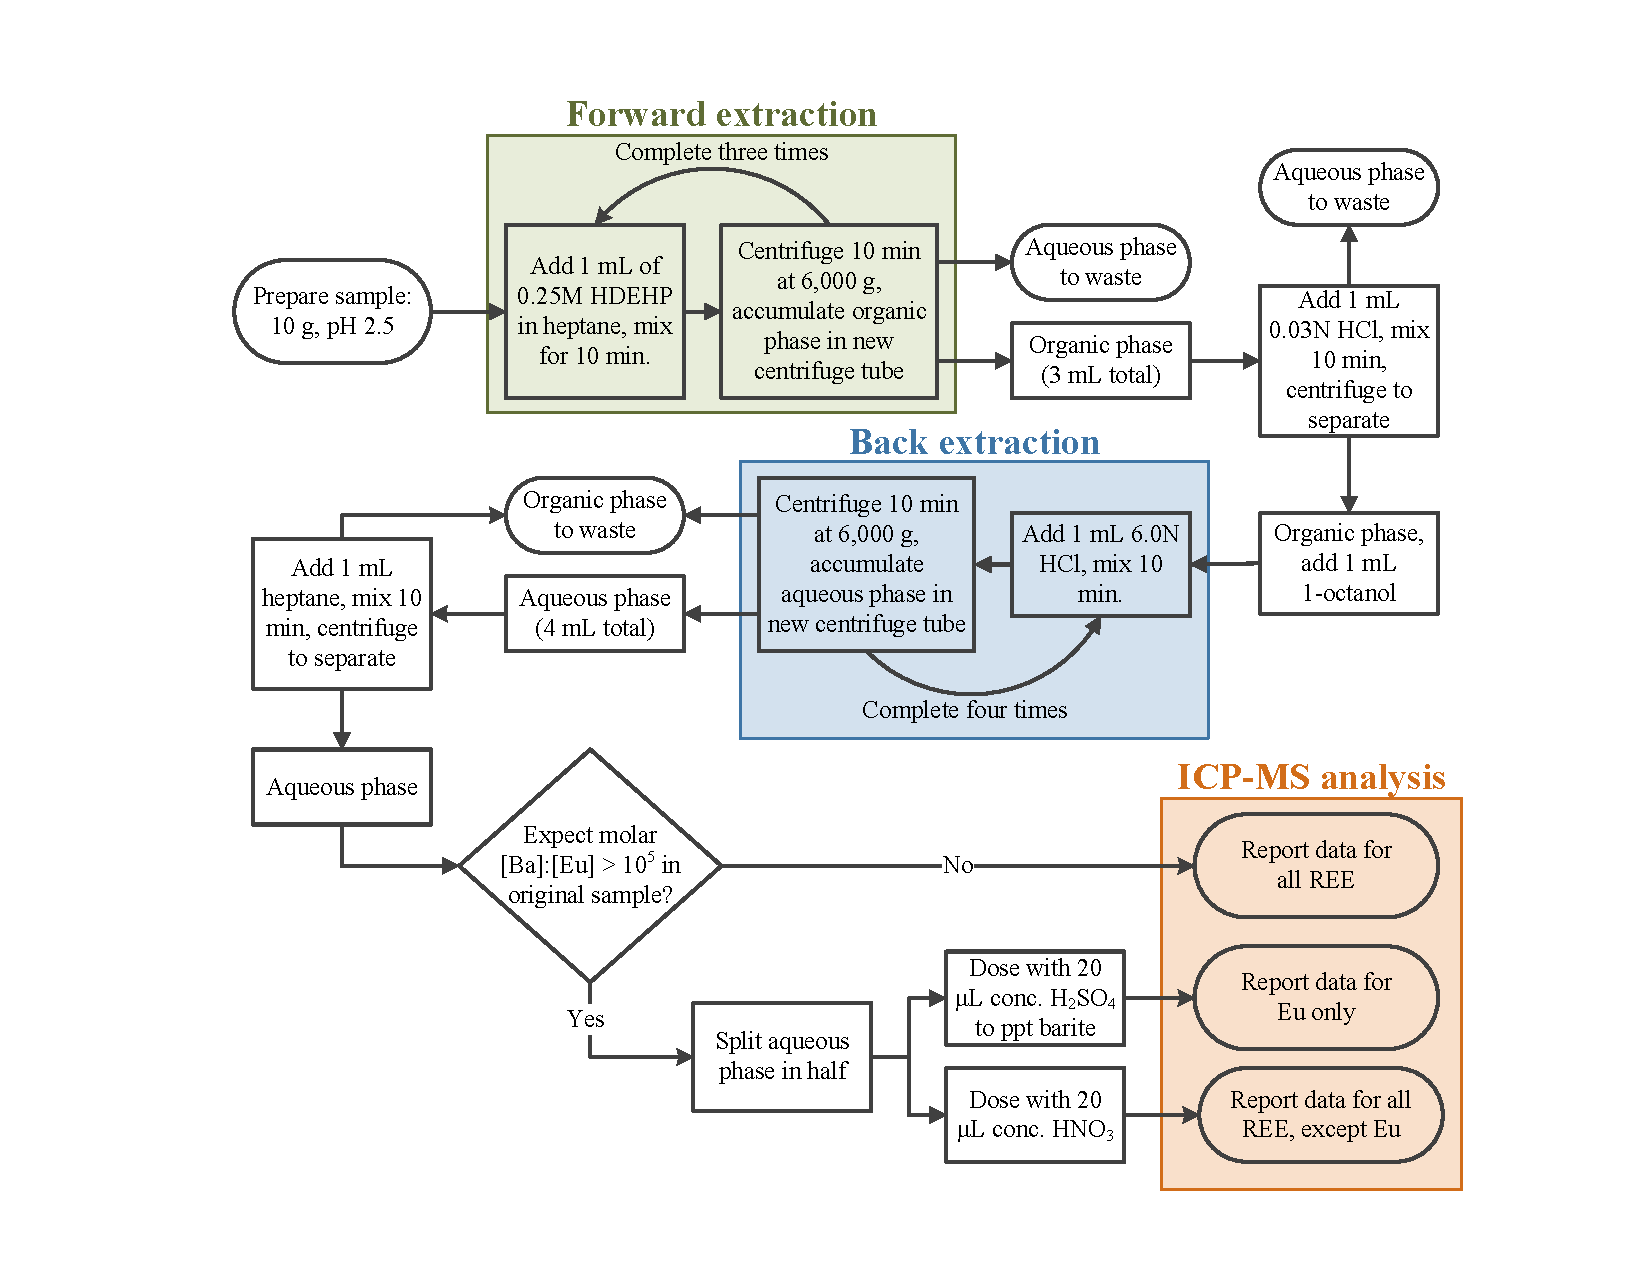
\includegraphics[width=0.8\textwidth]{Ch4_figures/LLE-flowsheet.pdf}
\caption{Liquid-liquid extraction method flowsheet for separation and concentration of REE from small volume, hypersaline brines. The decision node for the [Ba]:[Eu] molar ratio assumes a \ce{BaO+} formation rate on the order of 0.1\% in the ICP-MS.}\label{fig:flowsheet}
\end{center}
\end{sidewaysfigure}

Synthetic brine solutions were adjusted to pH 2.5 in 50 mL PP centrifuge tubes with \ce{HNO3} and subsequently split into 10 g aliquots in 15 mL PP centrifuge tubes for replicate experiments.
For each aliquot or sample, the process for REE extraction and recovery is as follows.
One (1) mL of 0.25 M HDEHP in heptane was added to the aqueous solution.
HDEHP was used as complexing agent for REE.
The phases were emulsified and mixed end over end for 10 minutes.
The phases were separated by centrifugation at 6,000$\times$g for 10 minutes and the light organic phase was removed from the centrifuge tube via pipette and accumulated in a new centrifuge tube, retaining the aqueous phase in the original tube.
This process, whereby the REE are complexed with HDEHP and partitioned into the heptane (termed forward extraction), was completed a total of three times.
Following the third forward extraction, the aqueous phase was discarded.

To remove any matrix (Na, Fe, etc.) and interfering species (i.e. Ba) that partitioned during forward extraction, the accumulated organic phase (3 mL total) was rinsed with 1 mL of pH 1.5 HCl.
This mixture was emulsified and separated by the same methods as the forward extraction.
Once separated, the dense aqueous phase was removed via pipette and discarded.

A concentrated acid solution was used to dissociate the REE-HDEHP complexes and return the REE to an aqueous phase (termed back extraction).
To decrease the REE-HDEHP complexation strength and encourage complete recovery \citep{Shabani_AC_1990},
1 mL of 1-octanol was added to the organic phase.
Back extraction was achieved with four, sequential steps of stripping with 1 mL of 6.0 N HCl (collecting the eluted REE in a total of 4 mL acid).
As with the forward extraction, the sample was emulsified and mixed end over end for 10 minutes and then separated via centrifugation at 6,000$\times$g for 10 minutes.
After centrifugation the aqueous phase was removed via pipette and accumulated in a separate centrifuge tube, retaining the organic phase in the original tube.
Following the four back-extractions, the organic phase was discarded.

The collected acid volume (4 mL) was then rinsed with 1 mL of heptane to remove any dissolved organics from the aqueous phase.
Phase mixing and separation were accomplished in the same manner as all other steps.
Following centrifugation, the dense aqueous phase was removed and analyzed.

Preliminary experiments (Figure~\ref{fig:Ba-removal}) indicated that, while Ba was successfully removed in the course of the LLE ($>99.9\%$ average reduction) and the HEHe-mode collision cell in the ICP-MS was successfully limiting \ce{^{135}Ba^{16}O+} interferences with \ce{^{151}Eu+} (\ce{^{135}Ba^{16}O+}:\ce{^{135}Ba+} $\sim0.2\%$ on average), initial Ba concentrations were so high that ppb level, background Eu concentrations were observed (Figure~\ref{fig:REE-bkgd}).
Thus, in order to determine Eu accurately in these synthetic brines an additional step was tested, where an aliquot of the final, collected acid volume was dosed with 20 \si{\uL} concentrated sulfuric acid (\ce{H2SO4}) to precipitate any remaining barium as barite (\ce{BaSO4}).
Efficiency of Ba removal after \ce{H2SO4} addition is compared in Figure~\ref{fig:Ba-removal}B and \ref{fig:Ba-removal}D.
It should be noted that this step was unnecessary for samples without Ba.

\begin{figure}[htbp]
\begin{center}
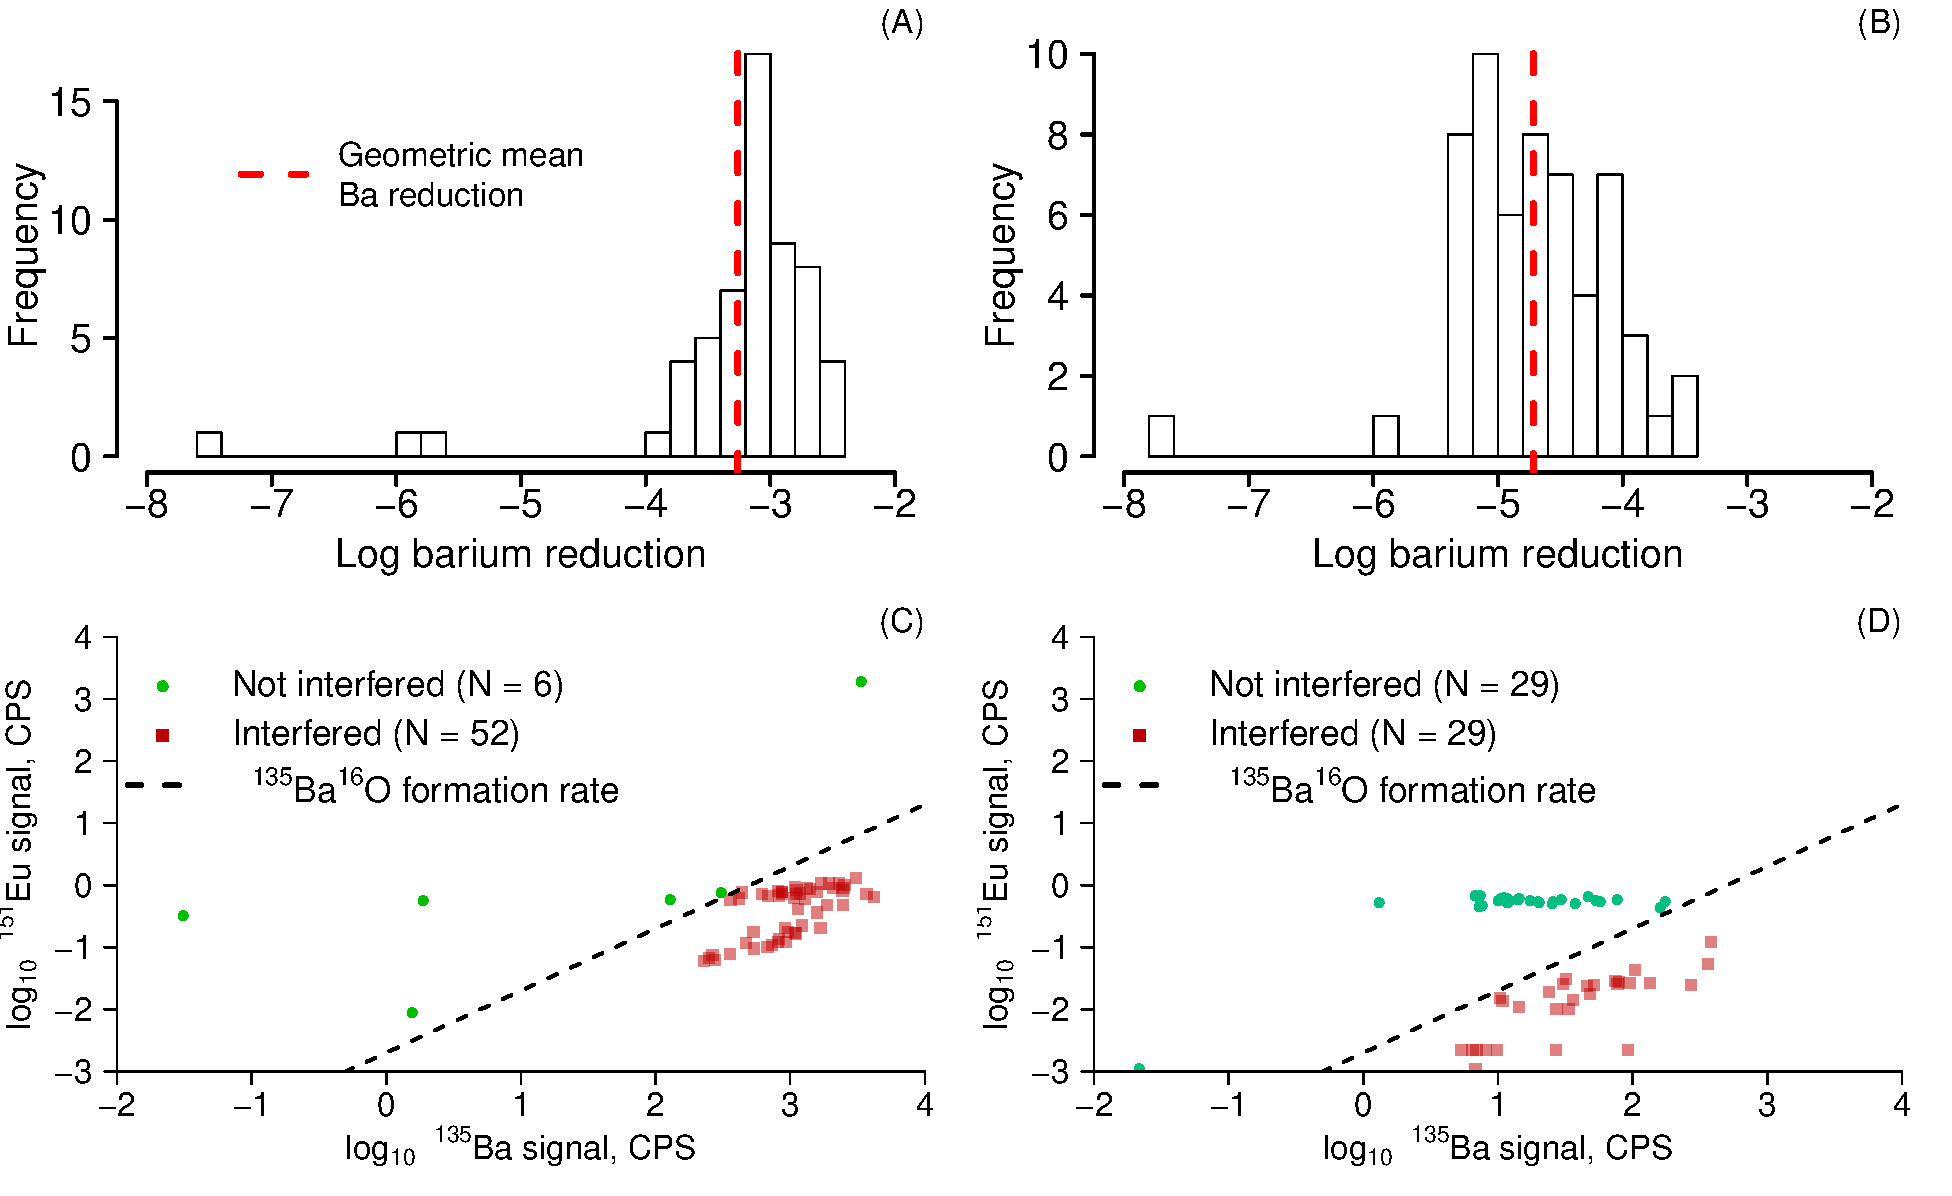
\includegraphics[width=\textwidth]{Ch4_figures/Ba-removal.pdf}
\caption{Efficiency of Ba removal by LLE method (A, C) and ICP-MS octopole collision cell (B, D).
Results are for samples without (A, C) and with (B, D) \ce{H2SO4} addition to precipitate barite.
In (B) and (D), \ce{^{135}Ba^{16}O+} rate is inferred from 23 replicate analyses of a 200 ppb Ba standard after blank subtraction.
Interfered samples are those where accurate Eu determination could not be made due to excessive \ce{^{135}Ba^{16}O+} interference. In (D) the interfered samples were all unspiked experiments.}\label{fig:Ba-removal}
\label{default}
\end{center}
\end{figure}

\begin{sidewaysfigure}[htbp]
\begin{center}
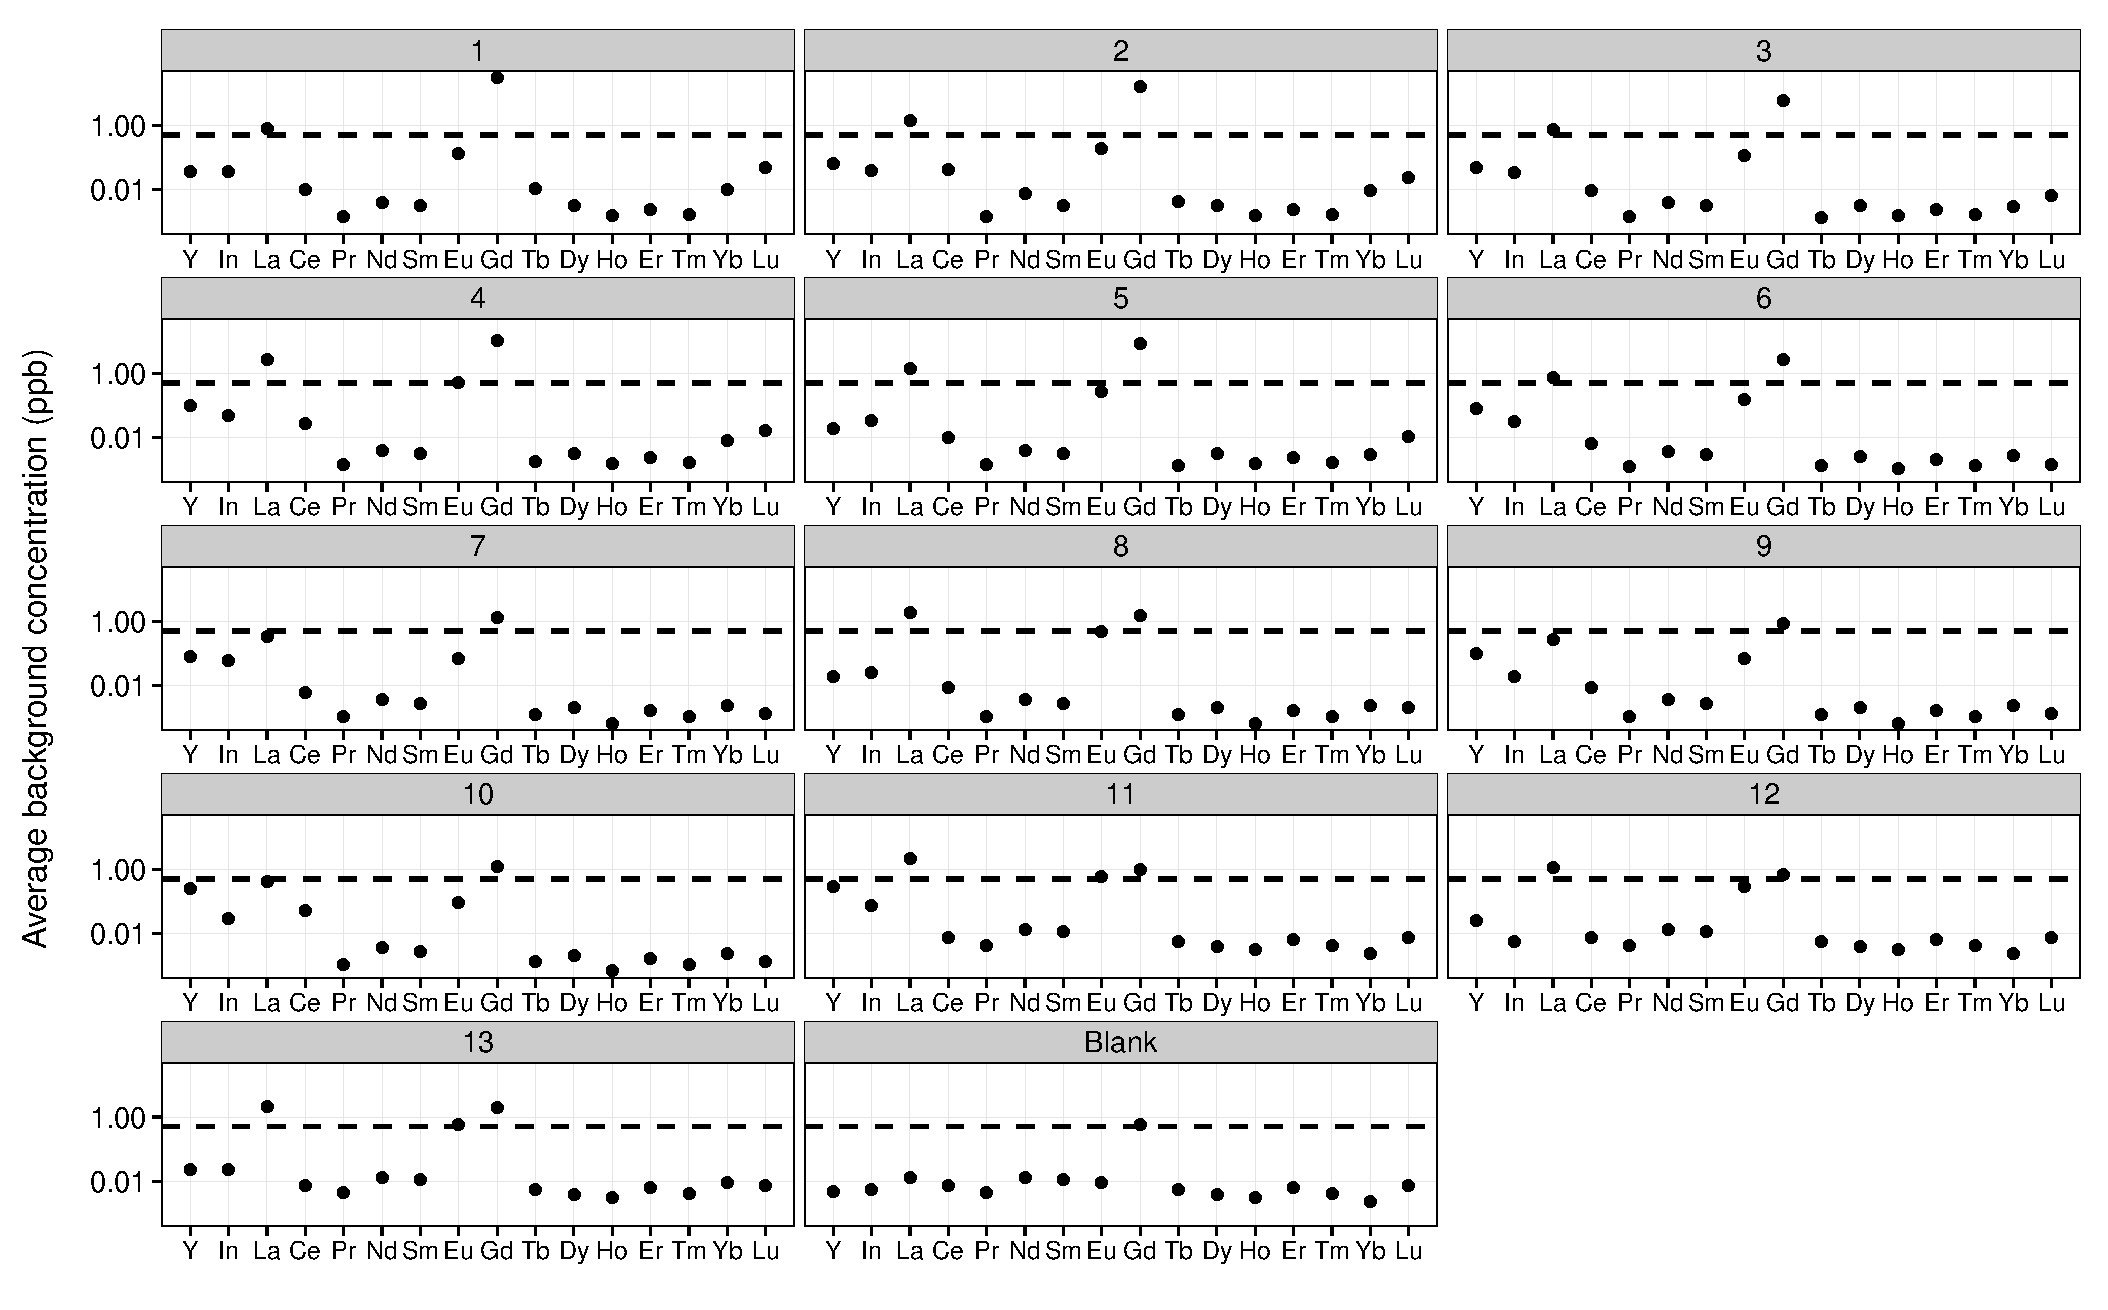
\includegraphics[width=0.9\textwidth]{Ch4_figures/REE-bkgd.pdf}
\caption{Average (from $n \geq 2$ replicates, except for Blank and experiments 6, 13) background concentrations of target analytes in samples without \ce{BaSO4} precipitation.
Dashed line at 500 ppt indicates the input concentration for all spiked samples.
Note that the y-axis is a logarithmic scale. Blank experiment represents pH adjusted ASTM Type I water.}\label{fig:REE-bkgd}
\end{center}
\end{sidewaysfigure}

The methodology of Jenner et al. \citep{Jenner_CG_1990} as modified by McGinnis et al. \citep{McGinnis_GN_1997} was employed to correct for matrix effects, isobaric interferences, and instrument drift during ICP-MS analysis.
For each sample a 2 mL aliquot was spiked with 2 mL of a mixed element standard (5\% \ce{HNO3} background) while a separate 2 mL aliquot was diluted with 2 mL of blank 5\% \ce{HNO3}.
These solutions were analyzed sequentially to examine sample-specific matrix effects and were followed by a 5\% \ce{HNO3} flush.
At the beginning of each analysis run and after every third sample, two separate standard solutions and an analytical blank were analyzed to monitor instrument drift and isobaric, polyatomic interferences (e.g. \ce{^{135}Ba^{16}O+} on \ce{^{151}Eu+} and light REE-oxides on heavy REE).
Eight, serially-diluted, multi-element standard solutions ranging in concentration from 50 ppt to 100 ppb were analyzed at the beginning and end of each run to confirm the linearity assumed by the internal/external calibration.
ypical analytical uncertainty was between 3 and 5\%.
Because of high backgrounds of Gd in our laboratory and high Ba in the experiments, oxide corrections for \ce{^{137}Ba^{16}O+} interference on \ce{^{151}Eu+} and \ce{^{157}Gd^{16}O+} on \ce{^{173}Yb+} were applied as in Aries et al. \citep{Aries_GN_2000} after ICP-MS analysis.

\section{Materials and methods}\label{sec:MnM}

\subsection{Chemicals and equipment}

For the LLE, n-heptane (Chromasolv\textsuperscript{\textregistered}; Lot \# SHBC0837V),
 1-octanol (Chromasolv\textsuperscript{\textregistered}; Lot \# SHBC6245V),
 and HDEHP (99.7\% purity; Lot \# MKBK0176V) were acquired from Sigma Aldrich.
 Nitric acid (\ce{HNO3}; BDH ARISTAR\textsuperscript{\textregistered} Plus, VWR; assay 69 wt.\%; Lot \# 1113050) was used for sample pH adjustment and as the solvent for all analyses.
 Hydrochloric acid (HCl; BDH ARISTAR\textsuperscript{\textregistered} Plus, VWR; 35 wt.\%; Lot \# 4113083) was used for matrix rinsing and REE back-extraction in the LLE.
 Chloride salts of Na (Sigma Aldrich; $\geq99\%$ purity), Ba (Alfa Aesar; $\geq 99.998\%$ purity), and Fe (Sigma Aldrich; $\geq 99.9\%$ purity, trace metal basis) and valeric acid (Alfa Aesar; 99\% purity) were used for preparation of synthetic brines.
 Single element standard solutions (1000 \si{\ug}/L) of the REE and all elements necessary for internal and external standardization were obtained from Inorganic Ventures.
 Polypropylene (PP) centrifuge tubes were used in the LLE and glass volumetric flasks were used to prepare organic phases.
Ultrapure water (ASTM Type I, 18.2 \si{M\ohm}/cm) was used for sample preparation and was prepared using a Barnstead NANOpure\textsuperscript{\textregistered} water purification system.
An OrionTM 8165BNWP ROSSTM Sure-FlowTM pH electrode (Thermo Scientific), coupled to an accumetTM XL600 meter (Fisher Scientific), was used for pH measurements of high-total dissolved solid (TDS) solutions.
The pH meter was calibrated with pH 2.0, 4.0, and 7.0 standards daily.
All samples were prepared gravimetrically using an analytical balance with 0.01 mg precision (Adam Equipment).

All analyses were performed on an Agilent 7700x ICP-MS with HEHe-mode octopole reaction cell.
Operating parameters were optimized daily via the auto-tune function of the Agilent MassHunter software using 1000:1 diluted Agilent tuning solutions;
typical operating parameters and monitored analyte masses are given in Table~\ref{tab:ICPMS}.

\begin{table}[htdp]
\caption{Typical operating conditions for ICP-MS analysis.
Analysis performed on Agilent 7700x using oxygen-free argon as the carrier and dilution gas and ultra high-purity helium in the reaction cell.
Conditions determined using 1000:1 diluted Agilent tuning solution.
For elements where multiple mass-to-charge ratios were monitored, \ce{^{148}Sm}, \ce{^{151}Eu}, and \ce{^{157}Gd} were used in data analysis.}\label{tab:ICPMS}
\begin{center}
\begin{tabular}{l l l}
\hline
 & Parameter & Value \\ \hline
 Plasma & & \\
  & RF power & 1600 W \\ 
  & Nebulizer pump rate & 0.10 rps \\
  & Carrier argon flow rate & 0.61 L/min \\ 
  & Dilution argon flow rate & 0.36 L/min \\ 
 Lenses & & \\ 
  & Extract 1 & 0.0 V \\
  & Extract 2 & -200.0 V \\
  & Omega bias & -110 V \\
  & Omega lens & 9.6 V \\
  & Cell entrance & -110 V \\
  & Cell exit & -150 V \\
  & Deflect & -74.8 V \\
  & Plate bias & -150 V \\
 Octopole reaction cell & & \\
  & Octopole bias & -100.0 V \\
  & Octopole RF & 200 V \\
  & He flow rate & 10 mL/min \\
  & Energy discrimination & 7.0 V \\
 Data aquisition & & \\
  & Replicates & 5 \\ 
  & Integration time & 0.3 s\\
 Masses monitored & & \\  
  & \multicolumn{2}{l}{\ce{^{45}Sc}, \ce{^{89}Y}, \ce{^{115}In}, \ce{^{135}Ba}, \ce{^{137}Ba}, \ce{^{139}La}, \ce{^{140}Ce},} \\ 
  & \multicolumn{2}{l}{\ce{^{141}Pr}, \ce{^{145}Nd}, \ce{^{147}Sm}, \ce{^{148}Sm}, \ce{^{151}Eu}, \ce{^{153}Eu},} \\ 
  & \multicolumn{2}{l}{\ce{^{157}Gd}, \ce{^{158}Gd}, \ce{^{159}Tb}, \ce{^{163}Dy}, \ce{^{165}Ho}, \ce{^{167}Er},} \\
  & \multicolumn{2}{l}{\ce{^{169}Tm}, \ce{^{173}Yb}, \ce{^{175}Lu}} \\
 Oxides and doubly charged & & \\  
  & \multicolumn{2}{l}{\ce{^{140}Ce^{16}O+}/\ce{^{140}Ce} $< 2.1\%$} \\ 
  & \multicolumn{2}{l}{\ce{^{140}Ce^2+}/\ce{^{140}Ce} $< 1.6\%$} \\ \hline
\end{tabular}
\end{center}
\label{default}
\end{table}%

\subsection{Recovery analysis by surrogate recovery}

In the absence of a high-salinity, certified reference material for REE, the IUPAC recommended methodology of surrogate recovery \citep{IUPAC} was used to study the recovery of REE by this LLE method.
Synthetic brine samples were either left blank or spiked with constant amounts of REE.
The difference in results between these samples yielded the mass of the spiked analytes recovered by the LLE method.
Additionally, indium was included in the spike solution as it is commonly employed as an internal standard for REE separation to monitor recovery \citep{Shabani_AC_1990,Zawisza_JAAS_2011}.
Data below the instrument detection limit (DL) were assigned a value of $0.5\times$DL for computation; this occurred for roughly 41\% of all the REE in the unspiked samples and 4\% in the spiked samples.

\subsection{Preparation of synthetic brines}

In addition to optimization of operating parameters, the methodology must be validated for complex brine solutions.
The complexity of the brine is a function of background salinity and interfering compounds (both inorganic and organic).
This was investigated in two stages.
First, simple solutions (1 m and 5 m NaCl) were used to evaluate feasibility.
Second, compositional complexity was explored via a uniform shell, or Doehlert, experimental design \citep{Doehlert}, varying NaCl, Fe, and dissolved organic carbon (DOC) concentrations.

The concentrations of background salinity and interfering compounds were chosen to match reported value ranges found in studies of produced waters from unconventional gas development in the Marcellus Shale \citep{Haluszczak_AG_2013, Barbot_EST_2013, Gregory_Elements_2011, Arvind_EST_2013, Vidic_Sci_2013},
however the range of compositions studied is similar to other deep, basinal brines \citep{Kharaka_REG_2000}.
Dissolved organic carbon was modeled with pentanoic (or valeric) acid, a common component of deep, saline brines \citep{Kharaka_REG_2000},
with representative metal-complexing functionality.
Additionally, organic acids have been shown to be a significant component of DOC in produced waters from the Marcellus Shale \citep{Wolford_PSU_2011}.
The parameters of interest --- concentrations of NaCl, Fe, and DOC --- were scaled linearly.
Experimental conditions for variability in salinity, Fe concentration, and DOC concentration are given in Table~\ref{tab:Doehlert}.
For all experiments the concentration of each REE (along with indium) was set at 500 ppt (parts per trillion), a value that falls between the 45th percentile (for Tm) and the 1st percentile (for La) of natural REE distributions in groundwater \citep{Noack_EST_2014}.
Total dissolved Ba was held constant at 2,000 ppm, roughly the average concentration observed by Barbot, et al. \citep{Barbot_EST_2013} for Marcellus Shale produced waters.
Results of these experiments were analyzed by multiple linear regression (MLR) to determine which parameters of the synthetic brine influenced the recovery most strongly.

\begin{table}[htdp]
\caption{Doehlert experimental design matrix for LLE validation in chemically complex brines.
Doehlert coding for each experiment are given in parentheses next to the parameter value.
All variables were varied arithmetically.} \label{tab:Doehlert}
\begin{center}
\begin{tabular}{cccc}
\hline
Exp. & [NaCl] (m) & [Fe] (ppm) & [DOC] (ppm-C) \\ \hline
1 & 2 (0) & 40 (0) & 200 (0) \\ 
2 & 3.5 (1) & 40 (0) & 200 (0) \\ 
3 & 2.75 (0.5) & 74.6 (0.866) & 200 (0) \\ 
4 & 2.75 (0.5) & 51.6 (0.289) & 363 (0.817) \\ 
5 & 0.5 (-1) & 40 (0) & 200 (0) \\ 
6 & 1.25 (-0.5) & 5.4 (-0.866) & 200 (0) \\ 
7 & 1.25 (-0.5) & 28.4 (-0.289) & 37 (-0.817) \\  
8 & 2.75 (0.5) & 5.4 (-0.866) & 200 (0) \\ 
9 & 2.75 (0.5) & 28.4 (-0.289) & 37 (-0.817) \\ 
10 & 1.25 (-0.5) & 74.6 (0.866) & 200 (0) \\ 
11 & 2 (0) & 63.1 (0.577) & 37 (-0.817) \\ 
12 & 1.25 (-0.5) & 51.6 (0.289) & 363 (0.817) \\ 
13 & 2 (0) & 16.9 (-0.577) & 363 (0.817) \\ \hline
\end{tabular}
\end{center}
\label{default}
\end{table}%

\subsection{Optimization of liquid-liquid operation parameters}

Preliminary experiments utilizing LLE conditions described by Shabani et al. \citep{Shabani_AC_1990} and Lawrence and Kamber \citep{Lawrence_GGR_2007} were unable to achieve high or consistent recovery of the REE (Figure~\ref{fig:reproduction}A,B).
These experiments showed recovery $<80\%$ for all elements in all replicates, with significant variability, as well as preferential recovery of the MREE over the L- and HREE.
It should be noted that both Shabani et al. \citep{Shabani_AC_1990} and Lawrence and Kamber \citep{Lawrence_GGR_2007} employed a mixture of mono- and di-ester phosphonic acids as the chelating ligand.
This ligand combination was also explored, however preliminary experiments provided poor results compared to the pure diester (HDEHP) under the same conditions and was not studied further.

\begin{figure}[htbp]
\begin{center}
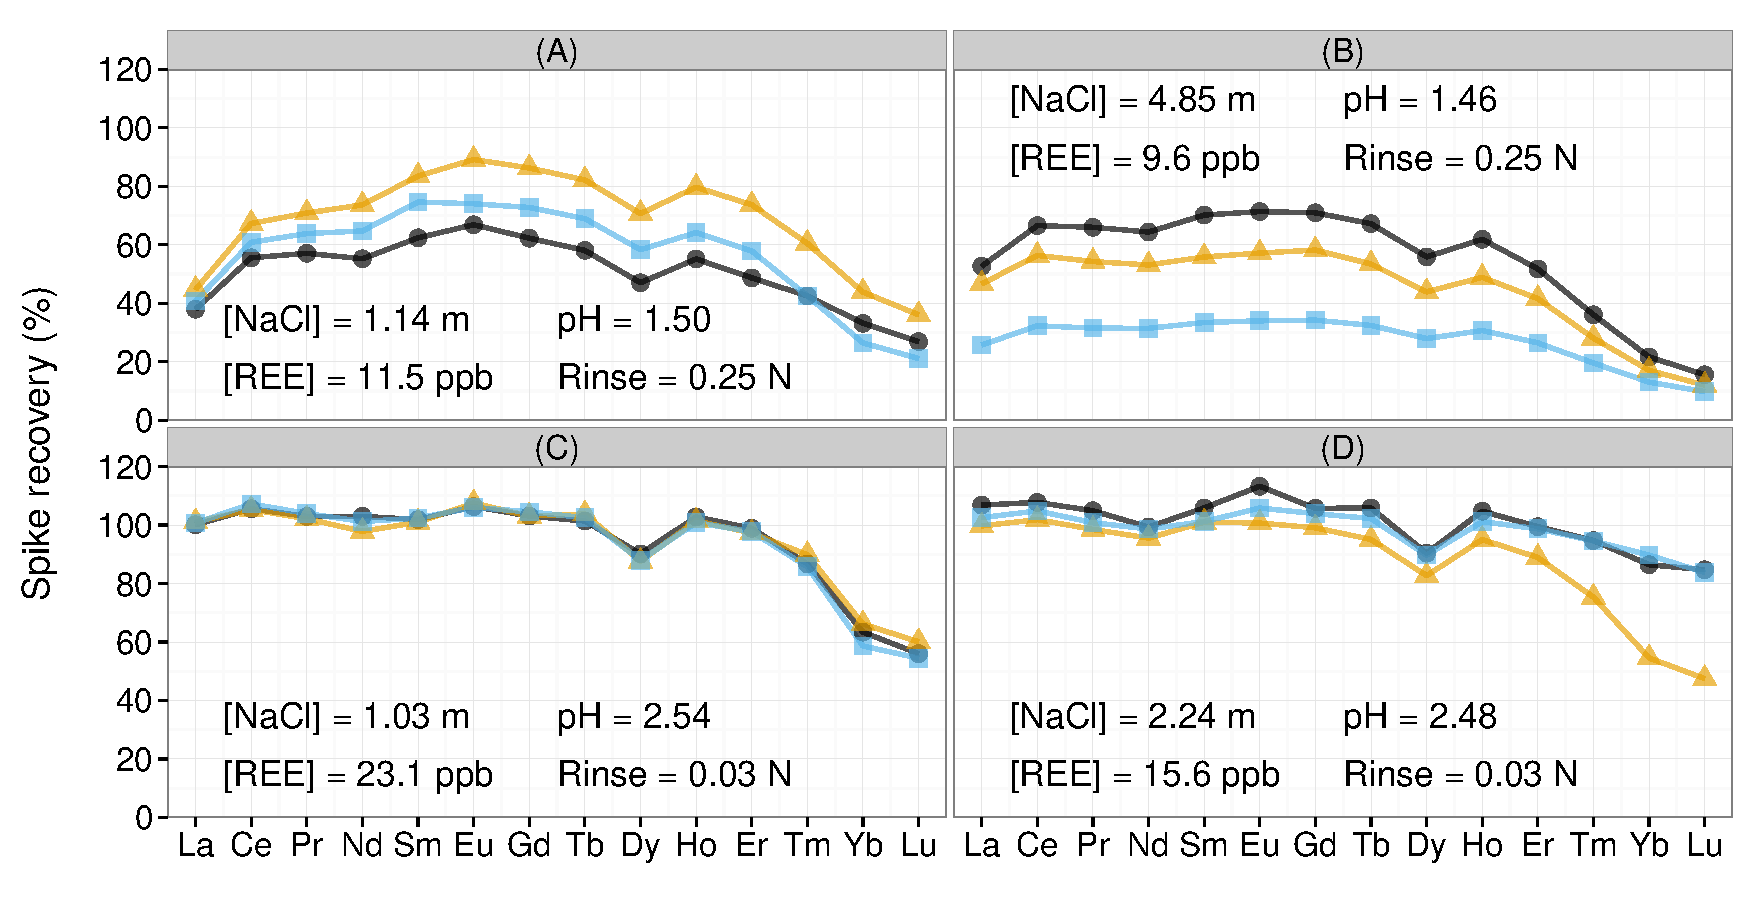
\includegraphics[width=\textwidth]{Ch4_figures/LLE-reproduction-recoveries.pdf}
\caption{REE recovery from 10 g samples of synthetic brine solutions using LLE conditions recommended by Shabani, et al.7 (A, B)
and ``optimal'' conditions predicted by multiple linear regression (C, D).
Each experiment was performed in triplicate (separate colors/shapes of plot) and the experimental conditions are shown in the subfigures.}\label{fig:reproduction}
\label{default}
\end{center}
\end{figure}

In order to optimize method performance, a linear model (Equation~\ref{eq:kimura_MLR}) was fit by ordinary least-squares in \texttt{R} \citep{R},
using the datasets of Kimura \citep{Kimura_BCSJ_1960, Kimura_BCSJ_1961}.
The relationship between the response (organic-aqueous distribution coefficient, $K_d$) and each of the predictors (solution acidity $[ACY]$, and ligand concentration $[L]$) is shown to be independently log-log linear.
Therefore the variables in this model correspond to log values. Data for fitting of this model were extracted from Figure 1 of Kimura \citep{Kimura_BCSJ_1960} for $K_d$ vs. $[ACY]$ at constant $[L]$ and from Figure 1 of Kimura \citep{Kimura_BCSJ_1961} for $K_d$ vs. $[L]$ at constant $[ACY]$. This estimation of parameter values reflects the dependence of $\log K_d$ on $\log[ACY]$ ($\beta_{ACY}$) and on $\log[L]$ ($\beta_L$) as well as a constant intercept ($\beta_0$).

\begin{align}\label{eq:kimura_MLR}
\log K_d = \beta_{ACY} \cdot \log[ACY] + \beta_L \cdot \log[L] + \beta_0
\end{align}

The extraction of REE from the aqueous to the organic phase is calculated using the predicted $K_d$ values based on mass balance.
The fraction of REE mass in the organic phase ($R_{org}$) for equilibrium between an aqueous phase (with volume $V_{aq}$) and an organic phase (with volume $V_{org}$) is calculated by Equation~\ref{eq:recovery}.

\begin{align}\label{eq:recovery}
R_{org} = \frac{1}{1 + \frac{V_{aq}}{V_{org}} \cdot K_d^{-1}}
\end{align}

The system can be represented as independent LLE in series since the phases are separated after each extraction step.
Thus, the overall partitioning of REE from the brine to the organic phase ($R_{tot}$) in the forward extraction can be calculated for $n$ sequential extractions with Equation~\ref{eq:step-recov}.
This allows for determination of the number of extractions necessary for quantitative recovery of REE.
The analysis is simply reversed to examine the elution properties of REE from the organic phase back into an aqueous phase.

\begin{align}\label{eq:step-recov}
R_{tot} = \sum_{i=1}^n R_{org}\left( 1 - R_{org} \right)^{i-1}
\end{align}

This analysis is meant to provide a ``best guess'' as to the optimal method parameters without requiring additional experimentation.
The inherent limitation of this approach is the uncertain extensibility of the original data to both a modified methodology (i.e. small volumes, changed organic diluent, mixed analyte solutions, low initial REE concentration) and unique matrices (i.e. acidified brines vs. HCl).
Therefore post hoc analysis of preliminary experiments for parameter optimization was done qualitatively and is described in Section~\ref{sec:param-adjust}. Moreover, since $K_d$ values were not calculated as part of this study, model validation with new experimental results was not performed.

\section{Results and discussion}

\subsection{Multiple linear-regression of organic-aqueous distribution coefficients} \label{sec:param-adjust}

Fractionation of the REE observed in preliminary experiments (Figures~\ref{fig:reproduction}A and \ref{fig:reproduction}B) can be qualitatively reconciled from MLR analysis.
Figure~\ref{fig:MLR-results} shows that the rinse step (labeled ``R'' in subfigures~\ref{fig:MLR-results}A to \ref{fig:MLR-results}D) creates strong stripping conditions ($\log K_d<-1$) for the LREE (La; Figure~\ref{fig:MLR-results}A) while the back extraction (labeled ``B'') may provide inadequate acidity to recover the HREE (Tm; Figure~\ref{fig:MLR-results}B) once partitioned.

\begin{sidewaysfigure}[htbp]
\begin{center}
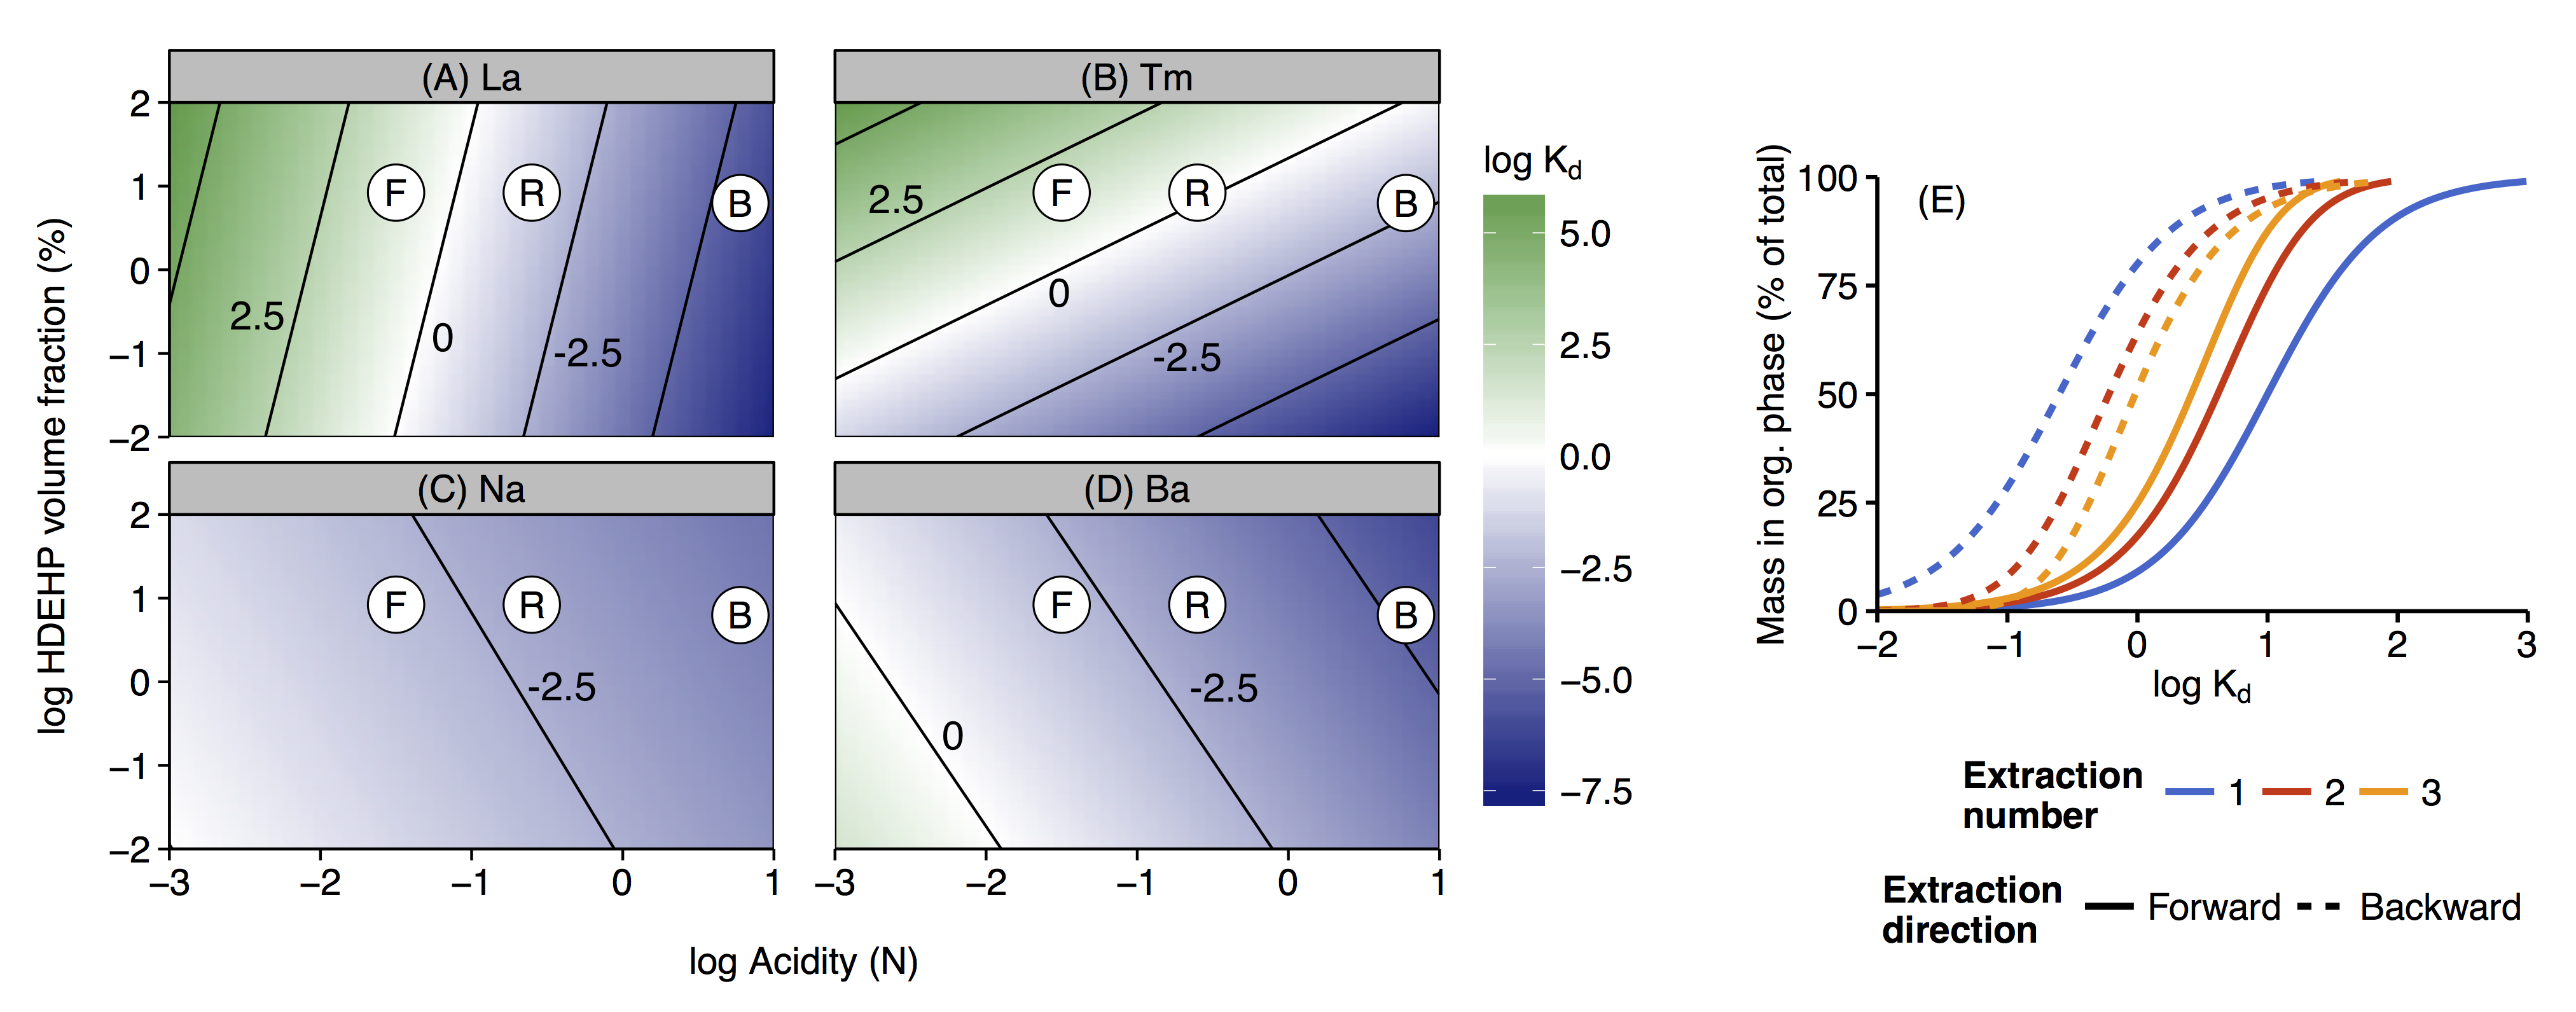
\includegraphics[width=\textwidth]{Ch4_figures/Kd-mod-plot.png}
\caption{Summary of model-based optimization of LLE operating conditions.
(A-D) Organic-aqueous distribution coefficient ($\log K_d$; Equation~\ref{eq:kimura_MLR}) contours as a function of acidity and HDEHP volume fraction for La, Tm, Na, and Ba calculated with data from Kimura \citep{Kimura_BCSJ_1960, Kimura_BCSJ_1961}.
LLE operating conditions for forward extractions (F), matrix rinse (R), and back extractions (B) suggested by Shabani et al. \citep{Shabani_AC_1990} are noted.
(E) Equilibrium partitioning for triplicate forward and backward extractions as a function of organic/aqueous distribution coefficient ($K_d$).
Partitioning calculated by Equation~\ref{eq:recovery} with $V_{aq}/V_{org} = 10$ for forward extraction and 0.25 for backward extraction.}
\label{fig:MLR-results}
\end{center}
\end{sidewaysfigure}


Using the equilibrium mass balance model (Equations~\ref{eq:recovery} and \ref{eq:step-recov}), the $K_d$ required to achieve the desired partitioning was matched to the results of this regression.
For each step of the LLE the desired partitioning is as follows:
\begin{enumerate}
	\item Forward extraction: Achieve high ($>99\%$) partitioning of the REE into the organic phase, while minimizing the partitioning of Ba and Na.
This can be achieved in a series of forward extractions.
	\item	Matrix rinse: Minimize partitioning of Ba and Na (i.e. low $K_d$) while maintaining a high ($>99\%$) partitioning of the REE. 
	\item Backward extraction: Minimize REE partitioning (i.e. leave $<1\%$ in the organic phase).
	This can be achieved in a series of backward extractions.
\end{enumerate}

Linear regression predicts a $\log_{10} K_d$ of 1.15 for La and 1.62 for Tm when using the conditions recommended by Shabani, et al.7.
At these values, a mass balance model would predict 93\% partitioning in three forward extractions for La and exactly 99\% for Tm.
Similarly, in the recommended matrix rinse (0.25 N HCl) the model predicts $\log_{10} K_d$ of $-1.48$ for La and 0.21 for Tm, which correspond to 9\% retention of La in the organic phase and 83\% retention of Tm.
While this simplified analysis suggests that triplicate back extraction steps should achieve quantitative recovery of all REE ($\log_{10} K_d$ of $-2.18$ and $-5.57$ for La and Tm respectively), preliminary experiments (Figure~\ref{fig:reproduction}C and \ref{fig:reproduction}D) showed that the HREE were incompletely recovered. From these results an additional elution step was added to the procedure. 

From this analysis, it is clear that the $K_d$ values need to increase for forward extraction and the matrix rinse in order to achieve the desired partitioning at each step.
The LLE conditions, namely the solution acidity $[ACY]$, necessary to meet these goals can be found be examining the contours of Figure~\ref{fig:MLR-results}A,B and E .
Using Figure~\ref{fig:MLR-results}E it can be shown that forward extractions require $\log K_d>1.6$ to achieve $>99\%$ partitioning to the organic phase after triplicate extractions. Further, the conditions of the rinse phase must maintain $\log K_d>1.4$  to retain $>99\%$ REE in the organic phase from one rinse step. Finally, to achieve $>99\%$ recovery of REE during triplicate back extractions, conditions must create $\log K_d<-1.2$.
By decreasing the initial acidity to $<10^{-2}$ N (i.e. pH $>2$) the initial extraction of REE can be enhanced without significantly increasing partitioning of Na or Ba. From this analysis, an initial sample pH of 2.5 was chosen.
At a pH of 2.5 ($[ACY] = 10^{-2.5}$ N), forward extraction yields $\log K_d$ of 4.1 and 3.2 for La and Tm respectively.
Dissolution of the organic phase, which has been shown to diminish partitioning, should be limited below pH 3.54
Similarly, by reducing the acidity of the rinse step to $\leq10^{-1.5}$ N (i.e. pH $\geq1.5$) salts such as Na and Ba (Figures~\ref{fig:MLR-results}C and \ref{fig:MLR-results}D) can be eluted while retaining the REE (Figure~\ref{fig:MLR-results}A and \ref{fig:MLR-results}B).

\subsection{Interferences of synthetic brine constituents}

Results for REE recovery from simple solutions of 1 and 5 m NaCl, the REE are presented in Figure~\ref{fig:NaCl-only}.
In the 1 m NaCl solution, REE recovery was consistently between 90 and 110\%, however, indium recovery was markedly lower: 76 and 81\% in duplicate experiments.
Similar results were observed in the high salinity test (5 m NaCl), except that the heaviest two lanthanides, Yb and Lu, were recovered at a much lower rate, averaging 82\% for Yb and 72\% for Lu.
As the matrix rinse and back extraction conditions were identical between the 1 m and 5 m NaCl experiments, the diminished recovery is likely an artifact of diminished forward extraction and thus an effect of the increased salinity.
Recovery of indium from the 5 m NaCl solution (mean, 76\%) matched the recovery observed in the 1 m NaCl solution indicating that this diminished recovery is likely not a function of the salt concentration, and is instead endemic to indium in this extraction.

\begin{figure}[htbp]
\begin{center}
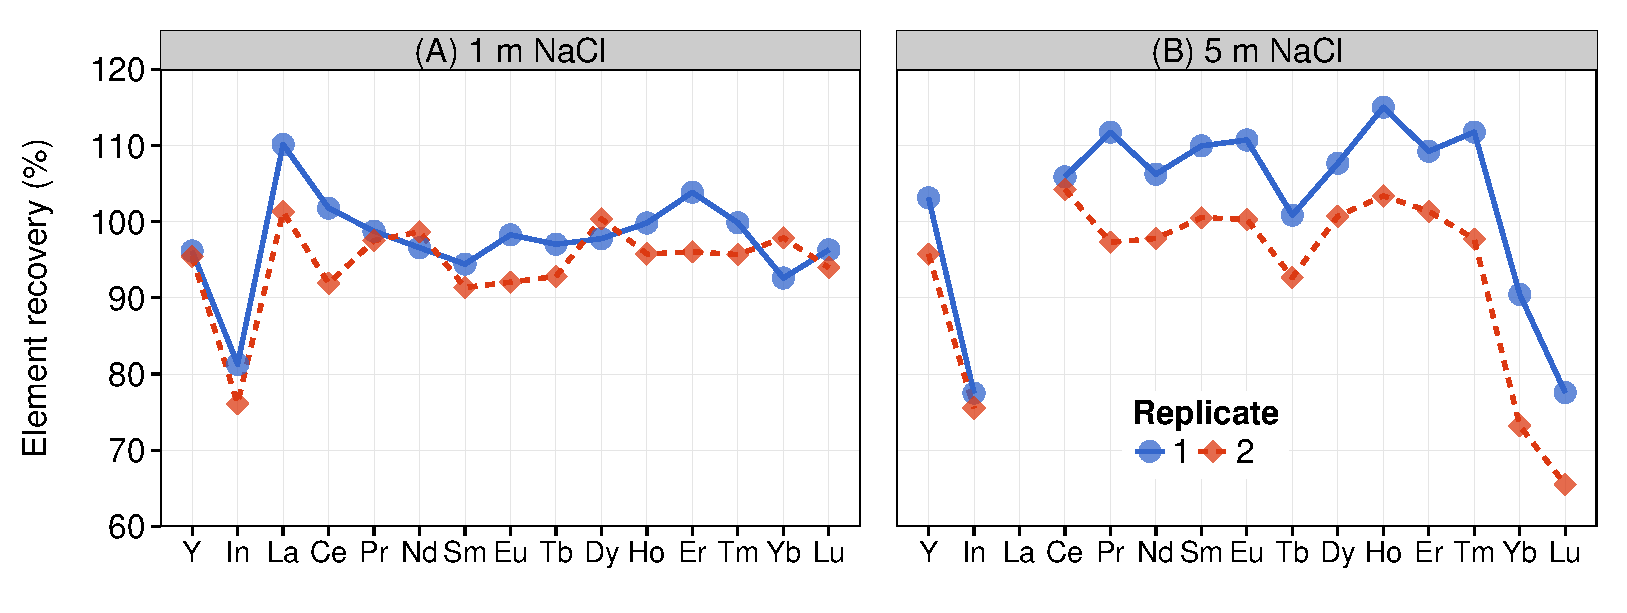
\includegraphics[width=\textwidth]{Ch4_figures/NaCl-only-LLE.pdf}
\caption{REE recovery by LLE method in simple, saline solutions.
Initial REE concentrations were 500 ppt (each element) in all experiments.
Duplicate experiments were conducted at each salinity and are represented by different line types, marker shapes, and colors.
Data for La in the 5 m NaCl experiment and for Gd in both experiments are excluded due to excessive background concentrations ($\geq250$ ppt).}
\label{fig:NaCl-only}
\end{center}
\end{figure}

Figure~\ref{fig:Doehlert-summary} summarizes the Doehlert design matrix experimental results, while experiment-ordered results, with replicates, are presented in Figure~\ref{fig:Doehlert-all}.
Data for Sc, La, and Gd are not included because these analytes were either not recovered (Sc, which is ``irreversibly bound'' in the organic phase \citep{Kimura_BCSJ_1960})
or contaminated by a high background (La and Gd; background $\geq 250$ ppt in all experiments).
Subsequent discussion excludes these elements.
Across all analytes, median recovery, $\widehat{Q}(0.50)=106\%$, was biased high (two-sided Wilcoxon Signed Rank test; H$_1$: $Q(0.5)\neq100\%$, $P < 10^{-6}$). However, these results are well within the recommended range of mean recovery for 1 ppb analytes (40 -- 120\% recommended) \citep{Taverniers_TrAC_2004}.
The absolute range of recoveries observed was 83-158\% while the reference range for recoveries (i.e the values between which 95\% of observations fell) was 92\% -- 122\%.
Experiments were generally reproducible (Figure~\ref{fig:Doehlert-all}), with element-specific, replicate standard deviations ranging from 0.05\% (Nd, experiment 4) to 21\% (In, experiment 1).
Finally, indium recovery was indistinguishable from any analyte (Wilcoxon, Rank-Sum test; $P>0.05$), in contrast to recovery from the simple NaCl solutions (Figure~\ref{fig:NaCl-only}).
Since these data are not sufficient to determine the mechanism by which this disparity was overcome, the application of indium as a tracer of REE recovery by the LLE method in unknown samples requires further study.

\begin{figure}[htbp]
\begin{center}
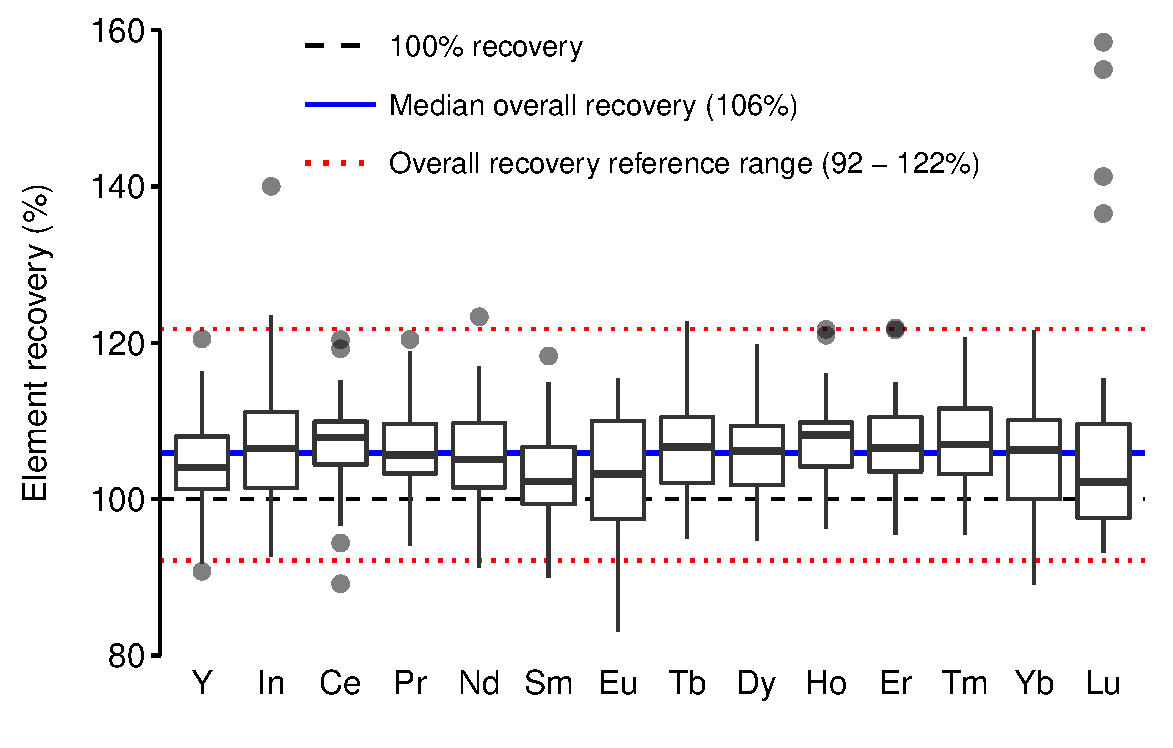
\includegraphics[width=0.8\textwidth]{Ch4_figures/Doehlert-results.pdf}
\caption{Distributions of elemental recovery in Doehlert matrix experiments by LLE methodology (see Figure~\ref{fig:Doehlert-all} for experiment-wise results). Distributions are depicted as standard box plots \citep{boxplots},
where the thick, black line depicts the median;
the boxed range represents the 25th to 75th percentile, or inter-quartile range (IQR);
the thin whiskers denote all measurements within 1.5 times the IQR above or below;
and the remaining observations are shown as semi-transparent grey dots.
Relevant summary statistics for the overall suite of analytes are given as horizontal lines.
Recovery values for Eu were determined after dosing the LLE eluent with \ce{H2SO4} to precipitate barite;
all other recoveries were determined without barite precipitation.
Data from La and Gd are not presented because the background concentration was determined to 250 ppt or greater (see Figure~\ref{fig:REE-bkgd}).}
\label{fig:Doehlert-summary}
\end{center}
\end{figure}

\begin{sidewaysfigure}[htbp]
\begin{center}
\includegraphics[width=\textwidth]{Ch4_figures/Exp-wise-LLE-recovery.pdf}
\caption{Elemental recovery in Doehlert matrix samples by LLE methodology (see Table~\ref{tab:Doehlert} for experimental conditions).
Recovery values for Eu were determined after dosing the LLE eluent with \ce{H2SO4} to precipitate barite;
all other recoveries were determined without barite precipitation.
Elements where the background concentration was determined to 250 ppt or greater (see Figure~\ref{fig:REE-bkgd}) were excluded (i.e. La and Gd in all experiments and Y in experiment 11).}
\label{fig:Doehlert-all}
\end{center}
\end{sidewaysfigure}

The data in Figures~\ref{fig:Doehlert-summary} and \ref{fig:Doehlert-all} indicate no clear fractionation (or mass bias) of the method across the suite of REE.
This result is confirmed by the Kruskal-Wallis test, which found no significant differences between any two element recoveries (H$_0$: No differences in element medians, $P > 0.1$).
Pairwise element testing (paired sample Wilcoxon Rank-Sum test, corrected for multiple comparisons) found statistically significant differences ($P < 0.05$) between 16 element pairs.
However, the differences were essentially indistinguishable from additive 3\% analytical errors (Figure~\ref{fig:element-diff-hist}).

\begin{figure}[htbp]
\begin{center}
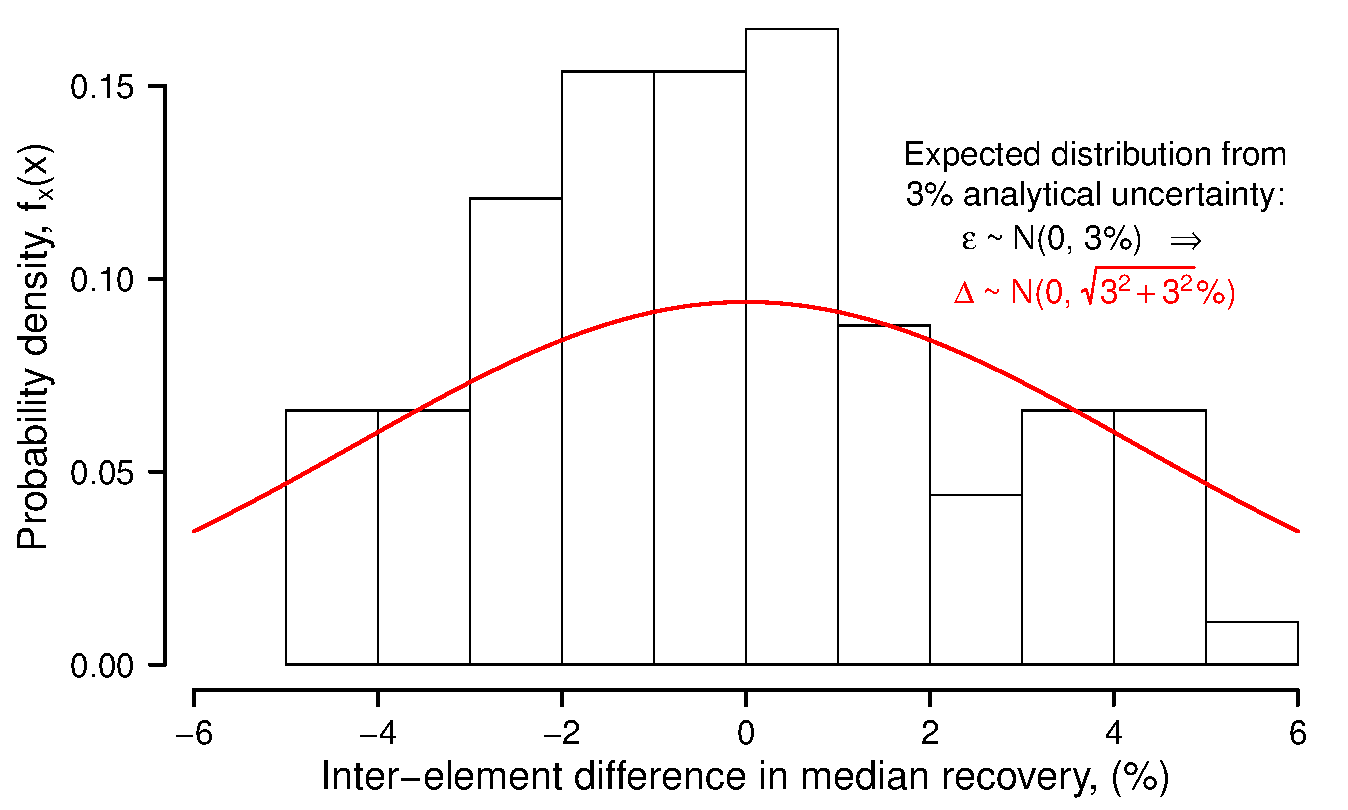
\includegraphics[width=0.75\textwidth]{Ch4_figures/element-diff-hist.pdf}
\caption{Comparison of pair-wise, inter-element differences in median recovery ($\Delta$, estimated from the paired-sample Wilcox signed rank test) to the expected (normal) distribution based on the difference between two random variates with equal means and 3\% analytical uncertainty, i.e.
$\Delta = N(\mu, 3\%) - N(\mu, 3\%) = N(0,\sqrt{3^2 + 3^2 }\%$).}
\label{fig:element-diff-hist}
\end{center}
\end{figure}


The lack of fractionation among REE in the more complex brines (i.e. with salinity, Fe, and DOC) differs from results obtained in experiments with simple NaCl solutions, where Yb and Lu recoveries were significantly lower at 5 m NaCl.
Step-wise regression analysis of element recovery (response) against solution composition (predictors) revealed no combination of linear- or interaction-terms among the study variables that substantially influenced recovery.
If the solution composition did have any impact on recovery within the range of parameters explored in the Doehlert design, it was indistinguishable from replicate variability.
These results give confidence to the application of the LLE methodology for natural samples with chemical characteristics within the bounds of the variables studied here, though accurate characterization of the REE concentration of unknown samples may require multiple replicates.

\bibliographystyle{unsrtnat}
\bibliography{Ch4_bib}
